\documentclass{article}
\usepackage[utf8]{inputenc}
\usepackage{url,amsmath,graphicx,amssymb,booktabs,adjustbox,subcaption,hyperref,float}
\usepackage[top=1.5cm, bottom=1.5cm, left=2.5cm, right=2.5cm]{geometry}
\usepackage{tikz}
\usetikzlibrary{positioning,shapes.multipart}

\newtheorem{theorem}{Theorem}
\newtheorem{lemma}{Lemma}
\newtheorem{corollary}{Corollary}
\newtheorem{definition}{Definition}
\newtheorem{Proposition}{Proposition}

\newcommand{\Prob}{\mathbb{P}}
\newcommand{\E}{\mathbb{E}}
\newcommand{\Space}{\mathbb{S}}
\newcommand{\Var}{\text{Var}}
\newcommand{\MR}{\mathcal{R}}
\newcommand{\MT}{\mathcal{T}}

\title{MA3676 -  2018 Past Paper}
\author{1720996}

\begin{document}
\maketitle
\tableofcontents
\pagebreak

\section{Safe Answers}
\begin{table}[h]
    \centering
    \begin{tabular}{|c|c|c|c|c|}
        \hline
        Question & & & Marks & Total Question Marks\\
        \hline
        1 & a & i & $[1]$ &  \\
         & & ii & $[3]$ & \\
         & & iv & $[4]$ & \\
         & & v & $[1]$ & \\
         & & vi & $[6]$ & \\
         & b & & $[3]$ & $18/20$ \\
         \hline
        2 & a & & $[4]$ & \\
         & b & & $[6]$ & \\
         & c & & $[3]$ & \\
         & d & & $[7]$ & $20/20$ \\
        \hline
        3 & a & i & $[10]$ & \\
         & & ii & $[3]$ & $13/20$\\
        \hline
        Best Score & & & & $51/60=$ A+ \\
        \hline
    \end{tabular}
    \label{tab:safe}
\end{table}

\section{1}
\subsection{a}
\subsubsection{i}
\begin{equation}
    \mathbf{p} = \begin{pmatrix}
        0 & \frac{1}{2} & 0 & \frac{1}{2} & 0 & 0 & 0 \\
        0 & 0 & 0 & 0 & 0 & 1 & 0 \\
        0 & 0 & \frac{3}{4} & 0 & \frac{1}{4} & 0 & 0 \\
        \frac{1}{4} & 0 & \frac{1}{4} & \frac{1}{4} & 0 & 0 & \frac{1}{4} \\
        0 & 0 & \frac{1}{2} & 0 & \frac{1}{2} & 0 & 0 \\
        0 & \frac{1}{2}  & 0 & 0 & 0 & \frac{1}{2} & 0 \\
        0 & 0 & 0 & 0 & 0 & 0 & 1
    \end{pmatrix}.
\end{equation}

\subsubsection{ii}
\begin{figure}[H]
    \centering
    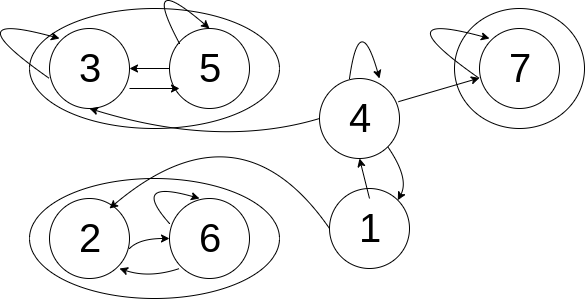
\includegraphics[scale=0.2]{diagram2018_1.png}
    \label{fig:1b}
\end{figure}
States $\{2,6\}$ and $\{3,5\}$ are ergodic closed recurrent sets, $\{7\}$ is absorbing and $1,4$ are transient. PQR decomposition can be done trivially.
\begin{equation}
    \mathbf{p} = \begin{pmatrix}
        0 & 1 & 0 & 0 & 0 & 0 & 0 \\
        \frac{1}{2} & \frac{1}{2} & 0 & 0 & 0 & 0 & 0 \\
        0 & 0 & \frac{3}{4} & \frac{1}{4} & 0 & 0 & 0 \\
        0 & 0 & \frac{1}{2} & \frac{1}{2} & 0 & 0 & 0 \\
        0 & 0 & 0 & 0 & 1 & 0 & 0 \\
        \frac{1}{2} & 0 & 0 & 0 & 0 & 0 & \frac{1}{2} \\
        0 & 0 & \frac{1}{4} & 0 & \frac{1}{4} & \frac{1}{4} & \frac{1}{4}
    \end{pmatrix}.\label{p_ii}
\end{equation}

\subsubsection{iii}
There are three closed sets of recurrent states, so three of the seven eigenvalues will be equal to one. There are no periodic states so the other eigenvalues are all less than one in magnitude.

\subsubsection{iv}
Find the equilibrium state of the closed set by solving
\begin{equation}
    \begin{pmatrix}
    \pi_2 & \pi_6
    \end{pmatrix} = \begin{pmatrix}
    \pi_2 & \pi_6
    \end{pmatrix}\begin{pmatrix}
    0 & 1 \\ \frac{1}{2} & \frac{1}{2}
    \end{pmatrix},
\end{equation}
to give you 
\begin{equation}
    \pi_2 = \frac{1}{3} \quad \pi_6 = \frac{2}{3}.
\end{equation}
Therefore, our answer is $\pi_2 = \frac{1}{3}$. 

\subsubsection{v}
States $1,4$ are transient, so the answer is $0$.

\subsubsection{vi}


\subsection{b}
The transition matrix can be written as
\begin{equation}
    \begin{pmatrix}
        a & b & 0 & 0 \\
        c & d & 0 & 0 \\
        e & 0 & f & 0 \\
        0 & 0 & g & 0 
    \end{pmatrix},\label{1_b}
\end{equation}
where the bottom-right $2x2$-matrix is $\mathbf{Q}$. We use this to solve 
\begin{align}
    \mathbf{\mu} &= (\mathbb{I} - \mathbf{Q})^{-1}\mathbf{e} \\
     &= \begin{pmatrix}
         1-f & 0 \\
         -g & 1
     \end{pmatrix}^{-1}\begin{pmatrix}
         1 \\ 1
     \end{pmatrix}\\
    &= \begin{pmatrix}
        \frac{1}{1-f} & 0 \\
        \frac{g}{1-f} & 1
    \end{pmatrix}\begin{pmatrix}
        1 \\ 1
    \end{pmatrix} \\
    &= \begin{pmatrix}
        \frac{1}{1-f} \\ 1+\frac{g}{1-f}     
    \end{pmatrix}= \begin{pmatrix}
        1.4 \\ 1.6
    \end{pmatrix}.
\end{align}
Solving this gives you the values of $f=\frac{2}{7}$ and $g=\frac{3}{7}$. Looking at the transition matrix back in (\ref{1_b}), we can see that $g$ must be equal to one, and therefore the information given in this question is not reliable.

\section{2}
\subsection{a}
The one-step transition matrix of the scenario is 
\begin{equation}
    \begin{pmatrix}
        0.8 & 0.2 & 0 & 0 \\
        0.05 & 0.75 & 0.2 & 0 \\
        0.05 & 0 & 0.75 & 0.2 \\
        0.1 & 0 & 0 & 0.9 
    \end{pmatrix}.\label{2a}
\end{equation}
It has an equilibrial solution because there are less than two closed sets.

\subsection{b}
Let $\mathbf{\pi}=(\pi_1,\,\pi_2,\,\pi_3,\,\pi_4)$ be our steady state of the transition matrix (\ref{2a}). We then solve
\begin{equation}
    \mathbf{\pi}\begin{pmatrix}
        0.8 & 0.2 & 0 & 0 \\
        0.05 & 0.75 & 0.2 & 0 \\
        0.05 & 0 & 0.75 & 0.2 \\
        0.1 & 0 & 0 & 0.9 
    \end{pmatrix} = \mathbf{\pi}.
\end{equation}
We obtain the linear equations:
\begin{align}
    0.8\pi_1 + 0.05\pi_2 + 0.05\pi_3 + 0.1\pi_4 &= \pi_1 \\
    0.2\pi_1 + 0.75\pi_2 &= \pi_2 \\
    0.2\pi_3 + 0.75\pi_3 &= \pi_3 \\
    0.2\pi_3 + 0.9\pi_4 &= \pi_4.
\end{align}
These can be solved in terms of $\pi_4$ to give
\begin{equation}
    \mathbf{\pi} = \left(\frac{25\pi_4}{32},\,\frac{5\pi_4}{8},\,\frac{\pi_4}{2},\,\pi_4\right) = \pi_4\left( \frac{25}{32},\,\frac{5}{8},\,\frac{1}{2},\,1 \right).
\end{equation}
Using the fact that the magnitude of $\mathbf{\pi}$ is one, we solve the following
\begin{equation}
    \pi_4\left( \frac{25 + 20 + 16 + 32}{32} \right) = 1,
\end{equation}
to find
\begin{equation}
    \pi_4 = \frac{32}{93}.
\end{equation}
This gives us the final equilibrium as
\begin{equation}
    \mathbf{\pi} = \left( \frac{25}{93},\,\frac{20}{93},\,\frac{16}{93},\,\frac{32}{93} \right),
\end{equation}
showing that the unemployment rate in the long run is $\pi_1 = \frac{25}{93}\approx 0.269\ldots$.

\subsection{c}
Using transition matrix (\ref{2a}), we note the in-goings and out-goings at each employment bracket, as well as the percentage of each that is taken into account.
\begin{table}[H]
    \centering
    \begin{tabular}{|c|c|c|c|}
    \hline
        Employment & Distribution & Salary & In/Outgoing \\
        \hline
        Unemployed & $25/93$ & $1500$ & $-100\%$ \\
        Level $1$ & $20/93$ & $2000$ & $+10\%$ \\
        Level $2$ & $16/93$ & $4000$ & $+10\%$ \\
        Level $3$ & $32/93$ & $6000$ & $+10\%$ \\
        \hline
    \end{tabular}
    \label{2c}
\end{table}
Expand this and calculate total monthly income $\mathbf{I}$:
\begin{align}
    \mathbf{I} &= -\left( \frac{25\mathbf{N}}{93}\times 1500\times 1 \right) + \left( \frac{20\mathbf{N}}{93}\times 2000\times 0.1 \right) + \left( \frac{16\mathbf{N}}{93}\times 4000\times 0.1 \right) + \left( \frac{32\mathbf{N}}{93}\times 6000\times 0.1 \right) \\
    &= \frac{\mathbf{N}}{93}\left[ -37500 + 4000 + 6400 + 19200 \right]\\
    &= -\frac{7900\mathbf{N}}{93}.
\end{align}
The country's treasury makes a loss of $-\frac{7900\mathbf{N}}{93}$ marks each month.

\subsection{d}
We create a new transition matrix such that
\begin{equation}
    \mathbf{p} = \begin{pmatrix}
        0.6 & 0.4 & 0 & 0 \\
        0.04 & 0.76 & 0.2 & 0 \\
        0.04 & 0 & 0.76 & 0.2 \\
        0.1 & 0 & 0 & 0.9 
    \end{pmatrix},
\end{equation}
alongside a new tax rate to derive the following:
\begin{table}[H]
    \centering
    \begin{tabular}{|c|c|c|c|}
    \hline
        Employment & Distribution & Salary & In/Outgoing \\
        \hline
        Unemployed & $0.146$ & $1500$ & $-100\%$ \\
        Level $1$ & $0.244$ & $2000$ & $+7\%$ \\
        Level $2$ & $0.203$ & $4000$ & $+7\%$ \\
        Level $3$ & $0.407$ & $6000$ & $+7\%$ \\
        \hline
    \end{tabular}
    \label{2d}
\end{table}
where our new distributions are found using the same method as that in question $2$b (use an online calculator, I use \url{http://psych.fullerton.edu/mbirnbaum/calculators/Markov_Calculator.htm}). We then go through the same process as $2$c to find our new income $\mathbf{I} = 42.94\mathbf{N}$ marks each month. This is definitely beneficial to the country's income.

\section{3}
\subsection{a}
\subsubsection{i}
\begin{equation}
    \Prob[S_j] = \Prob[S_j\vert+1]\Prob[+1] + \Prob[S_j\vert+2]\Prob[+2].
\end{equation}
This can be rewritten and substituted to
\begin{equation}
    P_j = P_{j+1}\cdot\frac{2}{3} + P_{j+2}\cdot\frac{1}{3}.
\end{equation}
This then corresponds to the characteristic equation
\begin{align}
    1 &= \frac{2}{3}\lambda + \frac{1}{3}\lambda^2 \\
    0 &= \frac{1}{3}\lambda^2 + \frac{2}{3}\lambda - 1 \\
    &=(\lambda+3)(\lambda-1)
\end{align}
giving us the solutions $\lambda=-3,\,1$. The general solution is therefore given as
\begin{equation}
    P_j = A + B(-3)^j.
\end{equation}
The boundary conditions are when you are at position $k$, so $P_k=1$, and when you are about to go to $k$ from $k-1$, so $P_{k-1} = \frac{2}{3}$. This gives us two equations:
\begin{align}
    P_k &= A+B(-3)^k = 1,\\
    P_{k-1} &= A+B(-3)^{k-1} = \frac{2}{3}.
\end{align}
We can solve for $A$ and $B$ as follows:
\begin{align}
    P_k-P_{k-1} = B(-3)^k-B(-3)^{k-1} &= \frac{1}{3} \\
    -3B(-3)^{k-1} - B(-3)^{k-1} &= \frac{1}{3} \\
    -4B(-3)^{k-1} &= \frac{1}{3} \\
    4(-3)B(-3)^{k-1} &= 1 \\
    4B(-3)^k &= 1 \\
    B &= \frac{1}{4}(-3)^{-k}.
\end{align}
Substituting this back in gives us
\begin{align}
    P_k = A + \left(\frac{1}{4}(-3)^{-k}\right)(-3)^k &= 1 \\
    A + \frac{1}{4} = 1 \\
    A = \frac{3}{4}.
\end{align}
Therefore, our general equation is now
\begin{equation}
    P_j = \frac{3}{4} + \frac{1}{4}(-3)^{j-k}.
\end{equation}
As $P_j$ denotes the probability of stepping on $k$ from position $j$, we just need to calculate
\begin{equation}
    P_0 = \frac{3}{4}+\frac{1}{4}(-3)^{-k}.
\end{equation}
This is the answer.

\subsubsection{ii}
$Y_n$ is martingale defined as $Y_n = S_n +\beta n$. For this to be true, the following equation must hold (and is subsequently solved)
\begin{align}
     \mathbb{E}[Y_{n+1}\vert\{S_i\}_{i=0}^n] &= Y_n = S_n+\beta n,\\
     &=  \mathbb{E}[(S_n+X_{n+1} + \beta(n+1)],\\
     &= S_n + \frac{4}{3} + \beta n + \beta = S_n+\beta n,\\
\end{align}
which is rearranged to show $\beta=-\frac{4}{3}$.\\
Note, $ \mathbb{E}[X] = \frac{4}{3}$ is shown true through
\begin{align}
     \mathbb{E}[X] = \mathbb{P}[X=1]\cdot  1 + \mathbb{P}[X=2] \cdot 2,\\
     &= \frac{2}{3}\cdot 1 + \frac{1}{3}\cdot 2 = \frac{4}{3}.
\end{align}
\subsubsection{iii}
To find the expected time to stop, we use the optional stopping theorem, giving us $\E[Y_T] = Y_0$. Using the result from $P_0$, we can see 
\begin{align}
    \E[Y_T] &= \E[S_t+\beta T] \\
    &= \E[S_T] - \frac{4}{3}\E[T]] \\
    &= P_0k + (1-P_0)(k+1) - \frac{4}{3}\E[T] \\
    &=Y_0.
\end{align}
Note here that $Y_0 = S_0 - \frac{4}{3}(0) = 0$ by using $Y_n$ from the previous question. It then follows that
\begin{align}
    Y_0 &= P_0k + (1-P_0)(k+1) - \frac{4}{3}\E[T] \\
    0 &= P_0k + (1-P_0)(k+1) - \frac{4}{3}\E[T] \\
    \E[T] &= \frac{3}{4}(k+1-P_0) \\
    &= \frac{3}{4}\left(k + \frac{1}{4} - \frac{1}{4}(-3)^{-k}\right).
\end{align}

\subsection{b}
\subsubsection{i}


\subsubsection{ii}

\section{4}
\subsection{a}
As half the population have no offspring, we only want to be calculating results for the other half, note the first two lines and the change of starting point of the series. Therefore, we have the equation
\begin{align}
    1 &= \sum_{k=0}^\infty \Prob[X=k]\\
    &= \frac{1}{2} + \sum_{k=1}^\infty \Prob[X=k] \\
    \frac{1}{2} &= \left( \sum_{k=0}^\infty \Prob[X=k] - \sum_{k=0}^0 \Prob[X=k]\right) \\
    &= C\left( \sum_{k=0}^\infty \left(\frac{2}{3}\right)^k - \sum_{k=0}^0 \left(\frac{2}{3}\right)^k \right) \\
    &= C\left( \frac{1}{1-\frac{2}{3}} - 1 \right) \\
    \frac{1}{2}&= 2C \\
    C &= \frac{1}{4}.
\end{align}
This change in scheme is present throughout the question, so be aware.

\subsection{b}
\begin{align}
    G(s) &= \frac{1}{2} + \frac{1}{4}\sum_{k=1}^\infty \left( \frac{2s}{3} \right)^k \\
    &= \frac{1}{2} + \frac{1}{4}\left( \sum_{k=0}^\infty \left( \frac{2s}{3} \right)^k - \sum_{k=0}^0 \left( \frac{2s}{3} \right)^k\right) \\
    &= \frac{1}{2} + \frac{1}{4}\left( \frac{1}{1-\frac{2s}{3}} - 1 \right) \\
    &= \frac{1}{2} + \frac{1}{4}\left( \frac{3}{3-2s} - \frac{3-2s}{3-2s} \right) \\
    &= \frac{1}{2} + \frac{1}{4}\left( \frac{3-(3-2s)}{3-2s}  \right) \\
    &= \frac{1}{2} + \frac{1}{4}\left( \frac{2s}{3-2s}  \right) \\
    &= \frac{1}{4}\left( 2 + \frac{2s}{3-2s} \right) \\
    &= \frac{1}{4}\left(\frac{6-2s}{3-2s} \right) \\
    &= \frac{3-s}{2(3-2s)}.
\end{align}

\subsection{c}
Make use of the fact $\E[X] = G^\prime(1) = G^\prime(s)\vert_{s=1}$. Use the quotient rule to solve.
\begin{align}
    E[X] &= \frac{1}{2}\cdot\frac{d}{ds}\left.\left( \frac{3-s}{3-2s} \right)\right\vert_{s=1} \\
    &= \frac{1}{2}\left.\left( \frac{-(3-2s)+2(3-s)}{(3-2s)^2} \right)\right\vert_{s=1} \\
    &= \frac{1}{2}\left( \frac{-1+4}{1^2} \right) \\
    &= \frac{3}{2}.
\end{align}

\subsection{d}
As $\E[X]>1$, the probability of extinction is equal to the smallest root of $G(\xi)=\xi$, which is strictly less than $1$.  

\subsection{e}
Using what was just stated:
\begin{align}
    \frac{3-\xi}{6-4\xi} &= \xi \\
    3-\xi &= 6\xi - 4\xi^2 \\
    4\xi^2 - 7\xi + 3 &= 0 \\
    (4\xi-3)(\xi-1) = 0
\end{align}
giving us roots $\xi=1,\,\frac{3}{4}$. The smallest root is the solution, begin $\xi = \frac{3}{4}$.

\subsection{f}
We have $Z_{n+1} = \sum_{i=1}^{Z_n}X_i$, where $X_i$ is the number of offspring of the $i$-th insect in the $n$-the generation. Therefore
\begin{align}
    \mathcal{G}_{n+1}(s) &= \E[s^{Z_{n+1}}] \\
    &= \E[s^{\sum_{i=1}^{Z_n}X_i}] \\
    &= \E[\prod_{i=1}^{Z_n}\E[s^{X_i}]].
\end{align}
Here, we make use of the fact $\E[s^X] = G(s)$ in order to then simplify to
\begin{align}
    \mathcal{G}_{n+1}(s) &= \E[\prod_{i=1}^{Z_n}G(s)]\\
    &= \E[G(s)^{Z_n}] \\
    &= \mathcal{G}_n(g(s)).
\end{align}

\subsection{g}
\begin{align}
    \xi &= \sum_{k+1}^\infty \Prob[X=k]\xi^k \\
    &= G(\xi).
\end{align}





\end{document}
